\documentclass[12pt]{article}

\usepackage{sbc-template}
\usepackage{graphicx,url}

\usepackage[portuges]{babel}
\usepackage{lmodern}
\usepackage[utf8]{inputenc}
\usepackage{amssymb,amsmath}
\usepackage[T1]{fontenc}
\usepackage{textcomp}
\usepackage{verbatim}
\usepackage{bold-extra}
\usepackage{minted} % colorir códigos fontes fontes (necessário a opçào para compilação -shel-scape)

% Caminhos das Imagens
\graphicspath{{images/}}

%%%%%%%%%%%%%%%%%%%%%%%%%%%%%%%%%%%%%%%%%%%%%%%%%%%%%%%%%%%%%%%%%%%%%%%%%%%%%%%%
% Comandos
\newcommand{\degree}{\ensuremath{^\circ}}
\makeatletter
\newcommand\tinyv{\@setfontsize\tinyv{6pt}{6pt}}
\makeatother

%%%%%%%%%%%%%%%%%%%%%%%%%%%%%%%%%%%%%%%%%%%%%%%%%%%%%%%%%%%%%%%%%%%%%%%%%%%%%%%%
\sloppy

\title{Instructions for Authors of SBC Conferences\\ Papers and Abstracts}

\author{Luciana P. Nedel\inst{1}, Rafael H. Bordini\inst{2}, Flávio Rech
  Wagner\inst{1}, Jomi F. Hübner\inst{3} }

\address{Instituto de Informática -- Universidade Federal do Rio Grande do Sul
  (UFRGS)\\
  Caixa Postal 15.064 -- 91.501-970 -- Porto Alegre -- RS -- Brazil
\nextinstitute
  Department of Computer Science -- University of Durham\\
  Durham, U.K.
\nextinstitute
  Departamento de Sistemas e Computação\\
  Universidade Regional de Blumenal (FURB) -- Blumenau, SC -- Brazil
  \email{\{nedel,flavio\}@inf.ufrgs.br, R.Bordini@durham.ac.uk,
  jomi@inf.furb.br}
}

%%%%%%%%%%%%%%%%%%%%%%%%%%%%%%%%%%%%%%%%%%%%%%%%%%%%%%%%%%%%%%%%%%%%%%%%%%%%%%%%

\begin{document}

\maketitle

\begin{resumo} 
	Realizar um Benchmark consiste em executar determinados processos em um computador, avaliando suas performances através da realização de vários testes. Neste artigo, vamos analisar um Benchmark realizado sobre as principais estruturas Java que implementam as interfaces \texttt{List}, \texttt{Set} e \texttt{Map}, sendo que todas fazem parte do Framework Collection.
\end{resumo}

\begin{abstract}
  Perform a Benchmark consists in run some computer process, evaluating their performances through performing several tests. In this paper, we are going to evaluate a benchmark accomplished on the main Java structures that implements the \texttt{List}, \texttt{Set} and \texttt{Map} interfaces, which are part of the Collection Framework.
\end{abstract}



\section{Descrição do Benchmark Criado} \label{sec:desc_bench}
	O trabalho desenvolvido, consiste em um benchmark de tempos de inserção de dez mil elementos aleatórios (gerados e armazenados previamente em arquivos), busca de cem elementos aleatórios na faixa de zero a dez mil (idem) e a remoção destes elementos, nas principais estruturas do Framework Collection do Java. As estruturas utilizadas foram: \texttt{ArrayList}, \texttt{Vector} e \texttt{LinkedList} (Interface \texttt{List}); \texttt{HashSet}, \texttt{LinkedHashSet} e \texttt{TreeSet} (Interface \texttt{Set}); \texttt{HashMap}, \texttt{LinkedHashMap} e \texttt{TreeMap} (Interface \texttt{Map}).\\
\subsection{A marcação do tempo}
	Para a realização da medição do tempo, uma classe \texttt{Benchmark} foi criada, de modo que possa ser extendida por qualquer outra, sendo portanto possível medir o tempo de execução de qualquer código. Assim, temos um método abstrato \textbf{exec()}, o qual será escrito pela classe que desejar utilizar-se deste Benchmark. A medição do tempo acontece ao chamar-se o método \textbf{start()}, o qual em seu interior marcará o início da contagem, executará o método \textbf{exec()} e marcará o final da contagem. O cógido abaixo tem a intenção de tornar mais clara toda esta ideia:\\
	\begin{minted}[linenos=true]{java}
public abstract void exec();

public void start() {
  time.init();
  exec();
  time.end();
}
	\end{minted}
	O objeto \textbf{time} da classe \texttt{Time} encarrega-se de marcar os tempos de relógio e cpu, do instante imediatamente anterior à execução e do posterior ao seu término.\\
\subsection{Executando e Salvando Resultados}
	O procedimento descrito a seguir foi realizado para todas as implementações do Framework Collection descritas no primeiro parágrafo desta seção.\\
	São gerados os arquivos especificados para a realização do benchmark e em seguida os valores neles contidos são utilizados para as operações de inserção, busca e remoção --- as quais se quer medir o desempenho. Esse procedimento é repetido \textsl{n} vezes, e na sequencia é tirada a média de cada tempo de cada estrutura. Estes resultados são então gravados em arquivos .dat que servirão para a construção dos gráficos.

\section{As Interfaces} \label{sec:interfaces}
	Interfaces formam o conjunto de interfaces disponíveis, onde Collections e todas as classes concretas irão derivar de uma ou mais interfaces.
	List e Set são um tipo de Collection, cada um com suas particularidades. Já um Map não é do mesmo tipo dos demais mas também manipula coleções de elementos.
	\subsection{List}
		Representa uma coleção ordenada (ordem de inserção) e que permite duplicatas, suas implementações são:
		\begin{itemize}
			\item[ArrayList:] Pode ser visto como um array (vetor) porém dinâmico. Ele é organizado pelo índice, ou seja, temos alguma garantia quanto a ordem que encontraremos os elementos.
			\item[Vector:] É basicamente um ArrayList, no entanto seus métodos são sincronizados o que significa que o acesso por vários processos simultaneamente é coordenado.
			\item[LinkedList:] Muito similar as duas coleções vistas anteriormente, porém todos os elementos são ligados entre si. Seu desempenho é superior aos do ArrayList e Vector quando necessitamos inserir elementos no início da coleção, no entanto ao precisar obter algum elemento pelo índice o desempenho é inferior.
		\end{itemize}
	\subsection{Set}
		Representa uma coleção que não pode conter duplicatas, implementa uma abstração dos conjuntos matemáticos, também contendo três implementações:
		\begin{itemize}
			\item[HashSet:] Caracteriza-se por não aceitar duplicatas, característica derivada do Set, ser uma coleção desordenada e desorganizada, isto é, não há nenhuma garantia quanto a ordem que os elementos serão percorridos.
			\item[LinkedHashSet:] É uma versão organizada do HashSet, ou seja, existe algum tipo de seqüência não-aleatória durante a iteração dos elementos, neste caso a ordem de inserção é respeitada. Por ser um Set, o LinkedHashSet não aceita duplicatas. Deve-se utilizar o LinkedHashSet ao invés do HashSet quando a ordem de iteração dos elementos é importante.
			\item[treeSet:] É um Set ordenado e como tal não aceita duplicatas, no TreeSet os elementos inseridos serão percorridos de acordo com sua ordem natural e de forma ascendente.
		\end{itemize}
	\subsection{Map}
		Implementa objetos que armazenam um elemento e o removem através da sua chave, não aceitam chaves duplicadas. Suas implementações são:
		\begin{itemize}
			\item[HashMap:] É um Map desorganizado, isto é, a ordem de iteração dos elementos é desconhecida, e desordenado.
			\item[LinkedHashMap:] É muito similar ao LinkedHashSet, porém esta é a versão que implementa a interface Map, logo ao armazenar os objetos é necessária uma chave. Ao contrário do HashMap, o LinkedHashMap é organizado, o que significa dizer que durante a iteração dos elementos ele respeita a ordem que estes foram inseridos na coleção.
			\item[TreeMap:] ordena seus elementos através da chave por alguma regra. Quando esta ordem não é definida pela interface Comparable ou por um objeto Comparator1 o TreeMap busca a ordem natural dos elementos.
		\end{itemize}


\section{Sobre os Benchmarks} \label{sec:bench}
	Na computação são necessários testes de hardware e software para gerenciamento de sua performance, esses testes são conhecidos como benchmarks. Benchmark é o ato de executar um programa de computador, um conjunto de programas ou outras operações, a fim de avaliar a performance relativa de um objeto, normalmente executando uma série de testes padrões e ensaios nele.

	Benchmark é útil para o entendimento de como o gerenciador de banco de dados responde sob a variação de condições. Pode-se criar cenários que testam o tratamento de deadlock, performance dos utilitários, diferentes métodos de carregar dados, características da taxa de transição quando mais usuários são adicionados e ainda o efeito na aplicação usando uma nova versão do produto.

\section{Gráficos dos Resultados}\label{sec:graphics}
	\begin{figure}[ht]
		\centering
		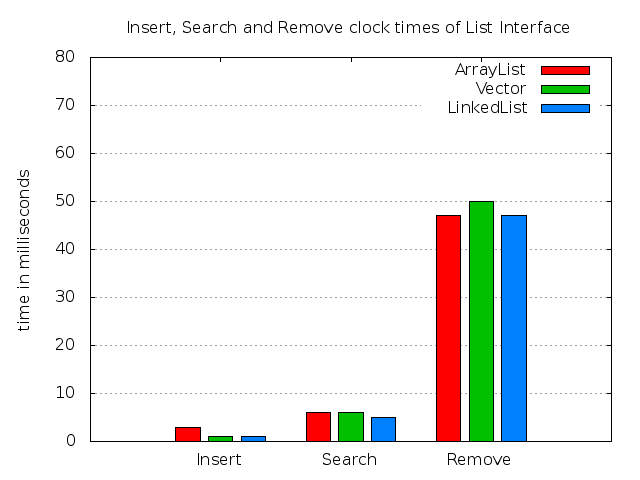
\includegraphics[width=.8\textwidth]{list_clock_graph.png}
		\caption{Interface List Clock times}
		\label{fig:list_clock}
	\end{figure}

	\begin{figure}[ht]
		\centering
		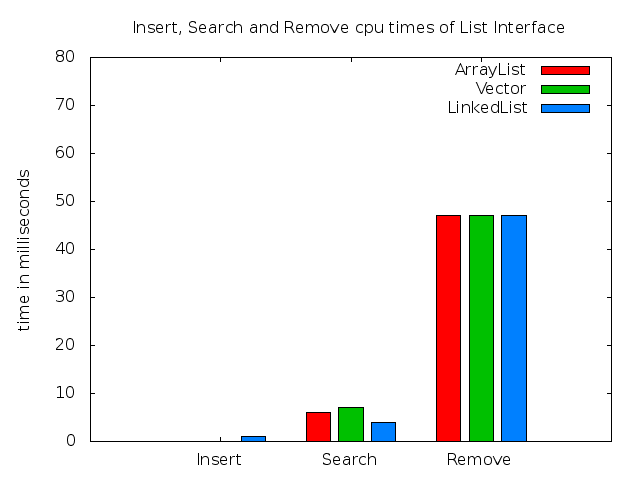
\includegraphics[width=.8\textwidth]{list_cpu_graph.png}
		\caption{Interface List Cpu times}
		\label{fig:list_cpu}
	\end{figure}

	\begin{figure}[ht]
		\centering
		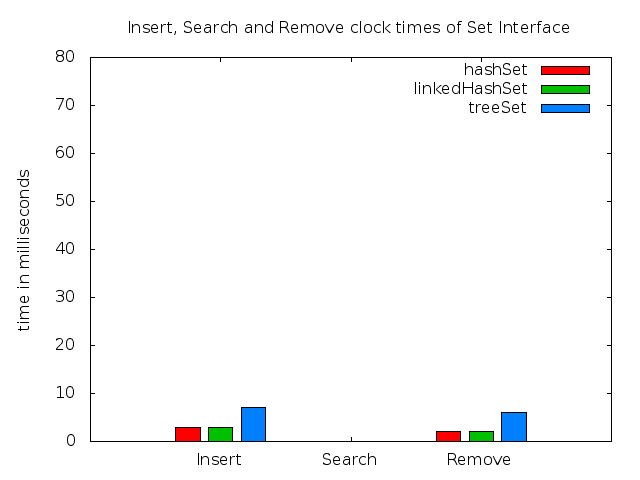
\includegraphics[width=.8\textwidth]{set_clock_graph.png}
		\caption{Interface Set Clock times}
		\label{fig:set_clock}
	\end{figure}

	\begin{figure}[ht]
		\centering
		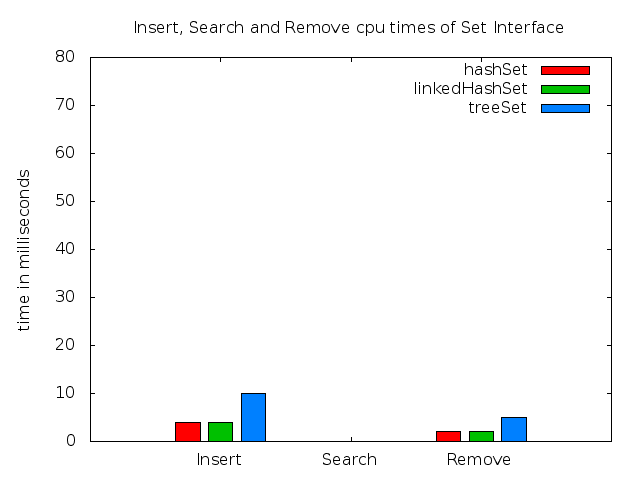
\includegraphics[width=.8\textwidth]{set_cpu_graph.png}
		\caption{Interface Set Cpu times}
		\label{fig:set_cpu}
	\end{figure}

	\begin{figure}[ht]
		\centering
		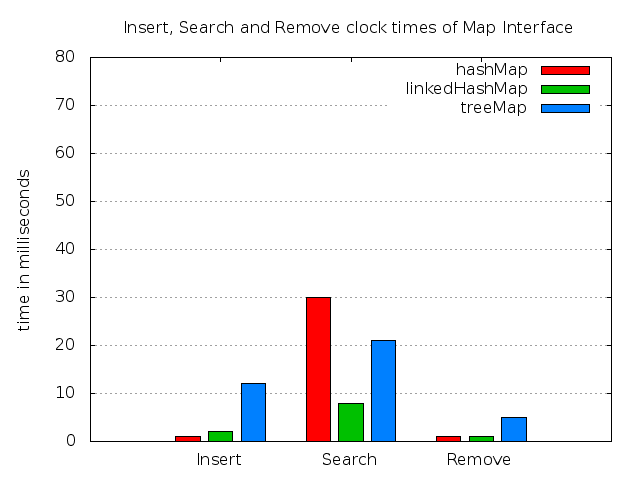
\includegraphics[width=.8\textwidth]{map_clock_graph.png}
		\caption{Interface Map Clock times}
		\label{fig:map_clock}
	\end{figure}

	\begin{figure}[ht]
		\centering
		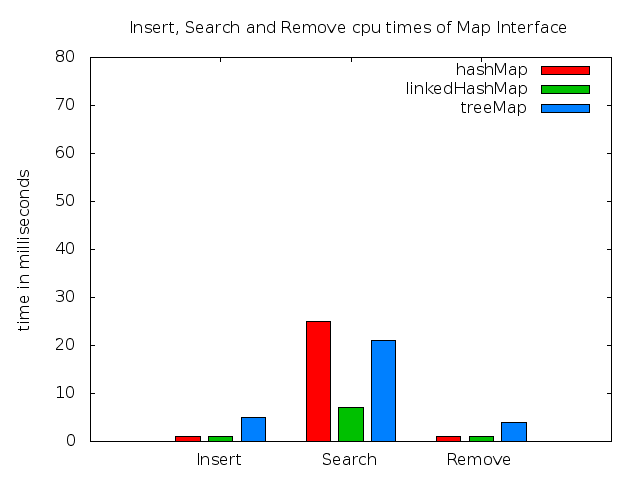
\includegraphics[width=.8\textwidth]{map_cpu_graph.png}
		\caption{Interface Map Cpu times}
		\label{fig:map_cpu}
	\end{figure}


\newpage
\section{Conclusão}\label{sec:conclusion}
	Com base nos fatos observados, podemos concluir que a estrutura que deveremos utilizar depende muito do nosso objetivo, visto que nenhuma é perfeita, mas cada uma tem suas peculiaridades, vantagens e desvantagens. Além disso, é importante citar que a obtenção e a análise dos resultados de benchmarks deve ser realizada com cautela, observando-se os vários fatores externos que podem eventualmente estar tendendo os mesmos para valores incorretos.

%\bibliographystyle{sbc}
\bibliography{bibliography/artigo}


\end{document}
